\documentclass[11pt, letterpaper]{article}
\usepackage[utf8]{inputenc}
\usepackage[letterpaper, margin=1in]{geometry}
\usepackage{amsmath}
\usepackage{amssymb}
\usepackage{amsthm}
\usepackage{graphicx}
\usepackage[font=scriptsize]{caption}
\usepackage{subcaption}
\graphicspath{ {./Report Images/} }
\captionsetup{justification=raggedright, singlelinecheck=false}
\usepackage{xcolor}
\usepackage{multicol}

\title{Project 1: Redwoods Data Report}
\author{Devin Ti and Ryan Tang}
\date{October 13th 2022}

\begin{document}
\maketitle

\section{Summary}
\subsection{Paper Overview}
The Redwoods paper demonstrated a case study by showing utilizing a sensor network enables a 
more in-depth analysis of any organism. With better technology, we can capture much more data in longitude and granularity than we previously could using a single, limited piece of equipment.
The motivation comes from numerous questions and requests from the local biologists. They have many intriguing things like studying, but the data availability hinders the observability and precludes
the possibility. The team decided on this study because the coastal redwood has a known micro-climate phenomenal variation within and across the days. It is the perfect subject for the demonstration and a great testbed to discover any limitations. With all these, the team showed that the newly acquired data reveals a much more complex dynamic system that Biologists have never been able to observe directly. The analysis also confirms that the redwood experiences substantial variation in temperature, moisture, and light levels throughout the day at its weather fronts.

\subsection{Data Collection}
The sensor network consists of 33 motes, a central network gateway, and an internal data logging backup. Each sensor is perfectly weathered while safely exposing the sensors, has its own battery, operating system, a top sensor for incident photosynthetically active radiation (PAR), and a bottom sensor for temperature, humidity, and reflected PAR. On average, they placed sensors across the entire redwood, mostly near the trunk and within a 1-meter radius, with 2-meter spacing. The placement started at the 15-meter mark and up to the pinnacle of the tree 67-meter. Such placement and spacing enable the sensors to capture the microclimate of the tree with the entire spectrum rather than the broader climate, which is our point of interest. One additional detail is that they placed most of their sensors on the west side of the tree because it has a ticker canopy to shield against environmental effects.

After nailing down the deployment plan, we have a few more things to confirm. The length of deployment is 44 days, starting on Tuesday, April 27th, 2004, at 5:10 pm and ending on Thursday, June 10th, 2004, at 2:00 pm. It also has a 5-minute sampling frequency. To put it precisely, it is up 4s every 5-minute to log the current sensor values, send it out through the network, and back to sleep again --- a 1.3\% duty cycle. In case of network failure, the readings were saved in the local logging system, which was retrieved after the experiment; however, it has a limited storage space and only works when the sensor battery is still up. 

The sensor cluster has an internal data collection framework, TinyDB. All data were collected through this framework using a SQL-like language and transmitted through the network most of the time. In particular, it retrieves four pertinent readings: relative humidity, temperature, incident PAR, and reflected PAR. In addition to the fours, it also records the nodeId, the parent nodeId, query time, and epoch. These are the relevant time and height dimensions used for keying purposes. 


\section{Data Cleaning}
\subsection{Data Description}
The data comes in two separate files.
\begin{enumerate}
    \item \textit{sonoma\_log} corresponding to measurements stored in the internal logging system of each sensor.
    \item \textit{sonoma\_net} corresponding to measurements stored in a network cloud system by each sensor.
\end{enumerate}
The two datasets correspond to how the data is collected. All sensors capturing a measurement at a given time attempt to write the measurement to a network database. Since the transmission might fail due to network issues, the sensor also writes the measurement to an internal database resulting in the log dataset. There are several implications of this process, and we will address them in the following sections.
\begin{enumerate}
    \item There are differences in how the various quantities are measured in the log and the network dataset. This is displayed in Figure \ref{fig1}, where histograms are plotted for the variables of interest. We have found that the differences are largely due to outliers.
    \item For a given sensor and a given time, there might be repeated measurements, one for the log and one for the sensor. In fact, we have found multiple sensors with multiple log and net readings at a given epoch. See Section 2.6 for details.
    \item Data yield is also a concern, The paper mentioned that have around 800k data point yield, but we only have around 415k data points in the given dataset after combining both the logged and network values. The actual effective yield is much lower due to duplicate or off measurements.
\end{enumerate} \\

\begin{figure}[!h]
\centering
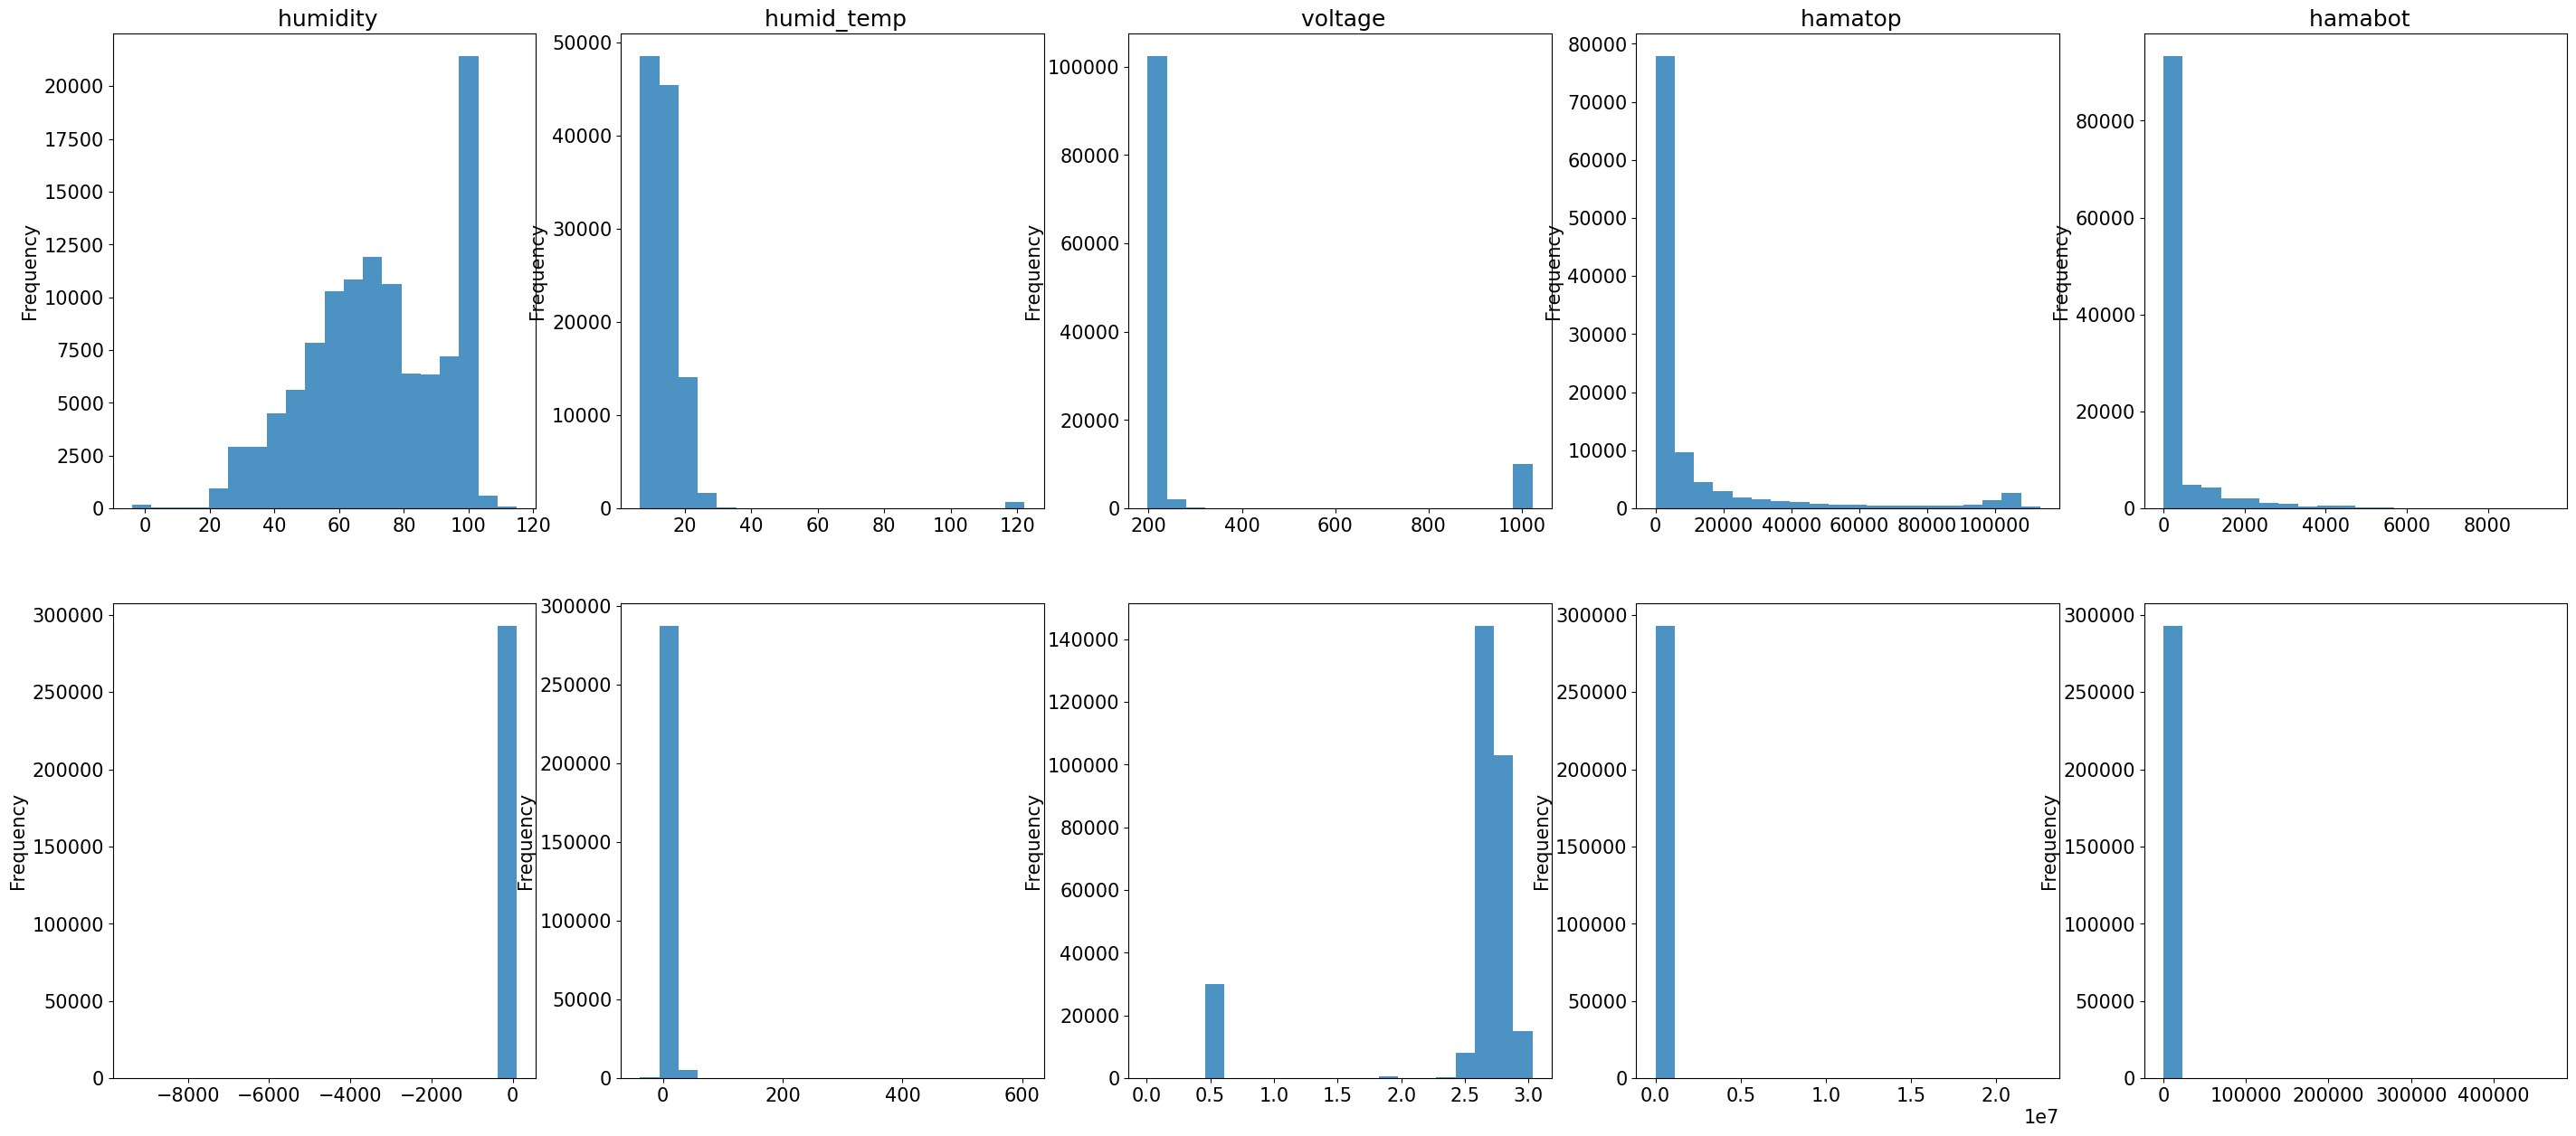
\includegraphics[width=1.0\textwidth]{Report Images/Fig1.png}
\caption{Histograms for 5 variables: humidity, temperature, voltage, incident PAR, reflected PAR. Top Row: Network data, Bottom Row: Log Data}
\label{fig1}
\end{figure}

\subsection{Part A: Histograms \& Converting Ranges}
Figure \ref{fig1} is meant to be compared to figure xx in the paper. This highlights two issues: 1) That the ranges of the data are not necessarily the same between the \textit{sonoma\_log} and the \textit{sonoma\_net} datasets, and 2) Some of the measurement units are different from that of the paper, as can be seen by the vastly different ranges. We see this in the PAR variables \textit{hamatop} and \textit{hamabot}. This is expressed in table x, where we plot several statistics for each variable of interest. Therefore, one should not concatenate the two files without any pre-processing.
\\ \\
We conducted two transformations:
\begin{itemize}
    \item For hamatop and hamabot in both datasets, we posit that the collected PAR number is under the unit of LUX, and we need to convert it down to $\mu mol/m^2/s$ by dividing it by $54$. 
    \item For voltage in \textit{sonoma\_net},  we convert xx
\end{itemize}
Fig xx and table xx show the statistics and histograms of the variables after the transformations. As we can see, the ranges of the two histograms are still not equal. This is due to outliers. We will address this in Part B.


\begin{figure}[h!]
\begin{tabular}{ |c|c|c|c|c|c| } 
    \hline & Median & Mean & SD & 25 Percentile & 75 Percentile \\ 
    \hline
    Humidity & 1 & 72.12 & 21.32 & 57.10 & 92.60 \\
    Temperature & 1 & 14.27 & 9.84 &	10.11  & 16.08\\
    Voltage & 1 & 292.79 & 227.22 & 218.0 & 227.0 \\
    Hamatop (incident PAR) & 1 & 11,521.65  & 24,962.81 & 0.0 & 8,436.36 \\
    Hamabot (Reflected PAR) & 1 & 271.94 & 805.30  & 0.0 & 0.0 \\
    \hline
\end{tabular}
\caption{Statistics for \textit{sonoma\_net} Pre-Transformation}
\end{figure}

\begin{figure}[h!]
\begin{tabular}{ |c|c|c|c|c|c| } 
    \hline & Median & Mean & SD & 25 Percentile & 75 Percentile \\ 
    \hline
    Humidity & 1 & 61.41  &	31.06 	& 40.02 	 & 80.19 \\ 
    Temperature & 1 & 15.02 	& 5.69 	& 10.86 	& 18.81 \\
    Voltage & 1 & 2.50 	& 0.64  & 2.62  & 2.77 \\
    Hamatop (incident PAR) & 1 & 10,870.34 & 48,422.14 & 0.0 & 6,762.33 \\
    Hamabot (Reflected PAR) & 1 & 245.53 & 1,180.33 & 0.0 & 0.0 \\
    \hline
\end{tabular}
\caption{Statistics for \textit{sonoma\_log} Pre-Transformation}
\end{figure}

\begin{figure}[h!]
\begin{tabular}{ |c|c|c|c|c|c| } 
    \hline & Median & Mean & SD & 25 Percentile & 75 Percentile \\ 
    \hline
    Voltage & 1 & ?& 227.22 & 218.0 & 227.0 \\
    Hamatop (incident PAR) & 1 & 213.36 & 462.27 & 0.0 & 156.22\\
    Hamabot (Reflected PAR) & 1 & 5.03	& 14.91 & 0.0 & 0.0 \\
    \hline
\end{tabular}
\caption{Statistics for \textit{sonoma\_net} after change of units}
\end{figure}

\begin{figure}[h!]
\begin{tabular}{ |c|c|c|c|c|c| } 
    \hline & Median & Mean & SD & 25 Percentile & 75 Percentile \\ 
    \hline
    Hamatop (incident PAR) & 1 & 201.302679 & 896.706333 & 0.00000 & 125.228333 \\
    Hamabot (Reflected PAR) & 1 & 4.546960 & 21.858109 &  0.00000 & 0.000000 \\
    \hline
\end{tabular}
\caption{Statistics for \textit{sonoma\_log} after change of units}
\end{figure}

\subsection{Part B: Missing Data}
There are also several sensors with missing data recorded in at least one of the 4 fields. We filter these data points out and present the statistics in Table \ref{table:data_info}. There are many lines with missing data, forming 2.746\% and 3.706\% of the log and network datasets, respectively.

\begin{figure}[h!]
\centering
\begin{tabular}{ |c|c|c|c|c| } 
    \hline & n Original & n After Missing Data Removed & n Missing & \% Missing \\
    \hline
    \textit{sonoma\_log} & 301,056 & 292,786 & 8,270 &2.746\\ 
    \textit{sonoma\_net}  & 114,980 & 110,718 & 4,262 & 3.706\\
    \hline
\end{tabular}
\caption{Size of log and network data sets, before and after missing data is removed.}
\label{table:data_info}
\end{figure}

\subsection{Part C: Location Auxiliary Data}
The next step is combining the measurements with the sensors' spatial information. This is done by joining the mote-location dataset with sonoma-log and sonoma-net on the ID and nodeid attributes, respectively. The resulting dataset has 14 columns each. Which are:
    \begin{multicols}{3}
    \begin{itemize}
        \item result\_time
        \item epoch
        \item nodeid
        \item parent
        \item voltage
        \item humidity
        \item humid\_temp
        \item humid\_adj
        \item Incident\_PAR(hamatop)
        \item Reflected\_PAR(hamabot)
        \item Height
        \item Direc
        \item Dist
        \item Tree
    \end{itemize}
    \end{multicols}

\subsection{Part D \& E: Outliers}
In this section, we further cleaned the data by removing outliers. We consider 2 types of outlier data measurements. 
\begin{enumerate}
    \item Outliers data measurements have abnormally high or low values of one of the variables of interest.
    \item Repeated measurements where a node has multiple measurements at a single epoch.
\end{enumerate}
Point 1. can be done in 2 ways. Firstly we combine the net and log data, threshold points are then set visually, and we classify data points beyond thresholds as outliers and remove them. To do this, we start off with the histogram in Figure \ref{fig3:combined_hist}. 

\begin{figure}[h!]
\centering
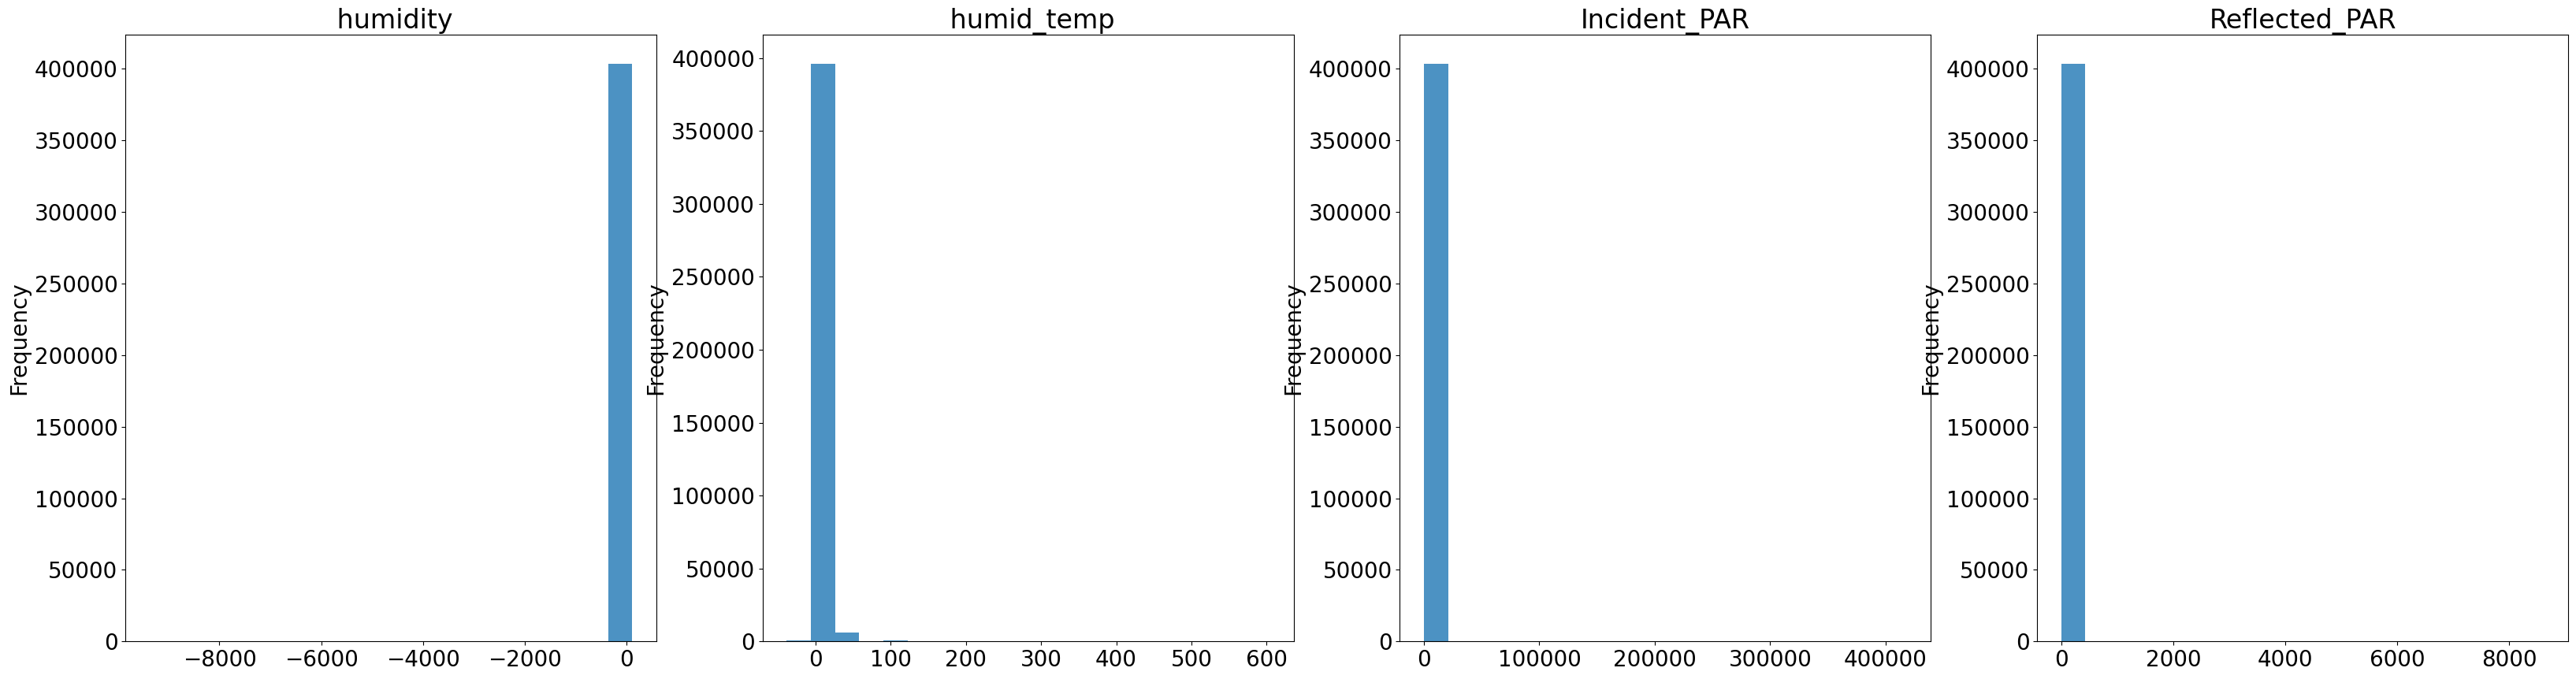
\includegraphics[width=1.0\textwidth]{Fig3_combined_hist.png}
\caption{Before the outlier removal}
\label{fig3:combined_hist}
\end{figure}

We set the following manual thresholds for the 4  variables, humidity, temperate, incident PAR, and reflected PAR.

\begin{itemize}
    \item humid: \textit{humid} $<$ 5
    \item Temperature: \textit{Temperature} $>$  140
    \item Incident\_PAR: \textit{Incident\_PAR} $>$  110000
    \item Reflected\_PAR: \textit{Reflected\_PAR} $>$  2000
\end{itemize}
In total, 864 points hit one of the conditions, with most data points (n=874) having a negative humidity. We further found that one data point is largely responsible for the large values in incident PAR and reflected PAR. After cleaning, the resulting histograms are shown in \ref{fig3:combined_hist_after_clean}. We can see that the histograms look much better, and the distribution of each variable is much more reasonable.

\begin{figure}[h!]
\centering
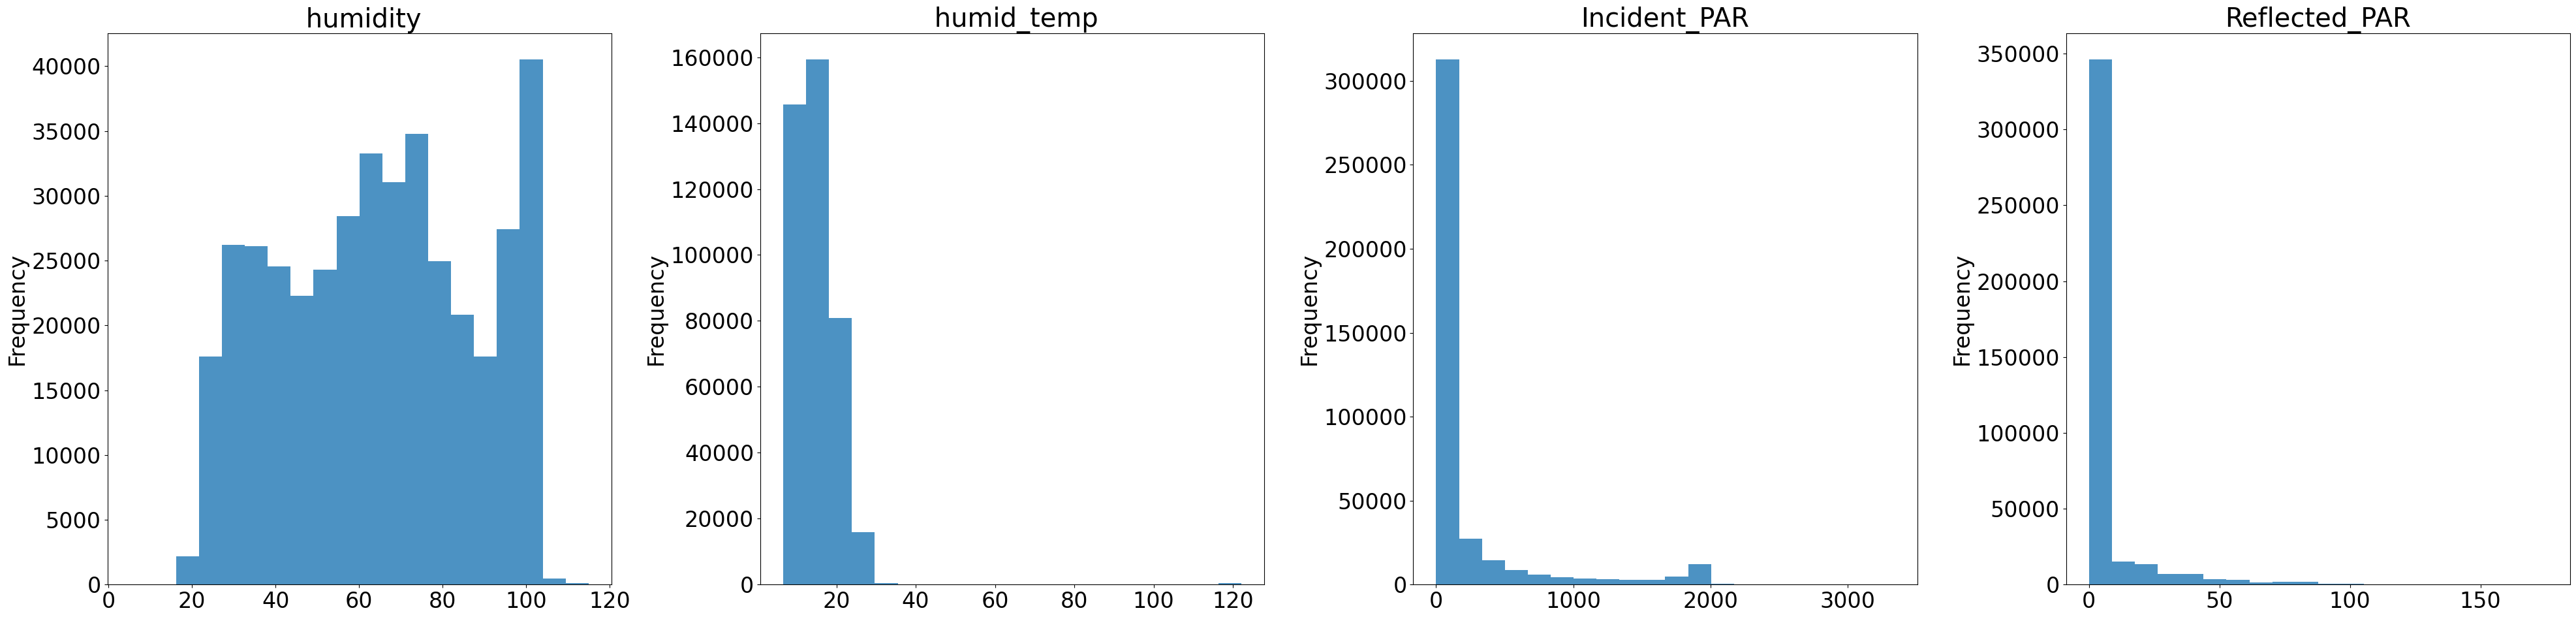
\includegraphics[width=1.0\textwidth]{Fig4_combined_hist_after.png}
\caption{After the outlier removal}
\label{fig3:combined_hist_after_clean}
\end{figure}


\subsection{Part E: Additional Pre-Processing}
We consider two additional cleaning measures. Removing readings at low voltages and removing repeated readings. With all the pre-processing, we end up with a dataset of $287,207$ in size.
\\ \\
\underline{Low Voltage}: The paper mentions that all readings taken where the node's voltage was outside of the range of 2.4 and 3 were removed. This range corresponds to the operational range of the sensor battery. If a sensor operates under a low battery condition, the outputting measurement is unreliable; thus, we can assume that readings taken outside this range have a high chance of being erroneous. As a first check, all outliers detected in Section 3.4 have voltages below 2.4, with the highest having 2.3291 volts and the lowest having 0.00906 volts. To keep in line with the paper, we removed an additional 28,699 data points where the voltage was outside $[2.4, 3]$.
\\ \\
\underline{Repeated Measurements}: As mentioned in Section xx. There are numerous data entries where the nodeid and the measurement epoch (time of measurement) are the same. This implies that exists multiple measurements for the same node at the same time period. We want to remove such duplicate entries because they can potentially skew the statistics and introduce un-welcomed bias. One way this duplication occurs is when both a log and a net value get saved for a given node and epoch. In total, there are $72,755$ node-epoch pairs where this duplication occurs. After inspecting these pairs, we find that the measurements are often the same, but there can be deviations in some cases. We also found that duplication can occur because the sensor writes multiple times in a short time to the network or to the log; this was the case for sensor nodeid 118. To de-duplicate, we take a random data point with a preference for the network measurements when all the measurements are the same. We take the smaller measurements if they are different. 


\section{Exploratory Data Analysis (EDA)}
\begin{figure*}[h!]
\centering
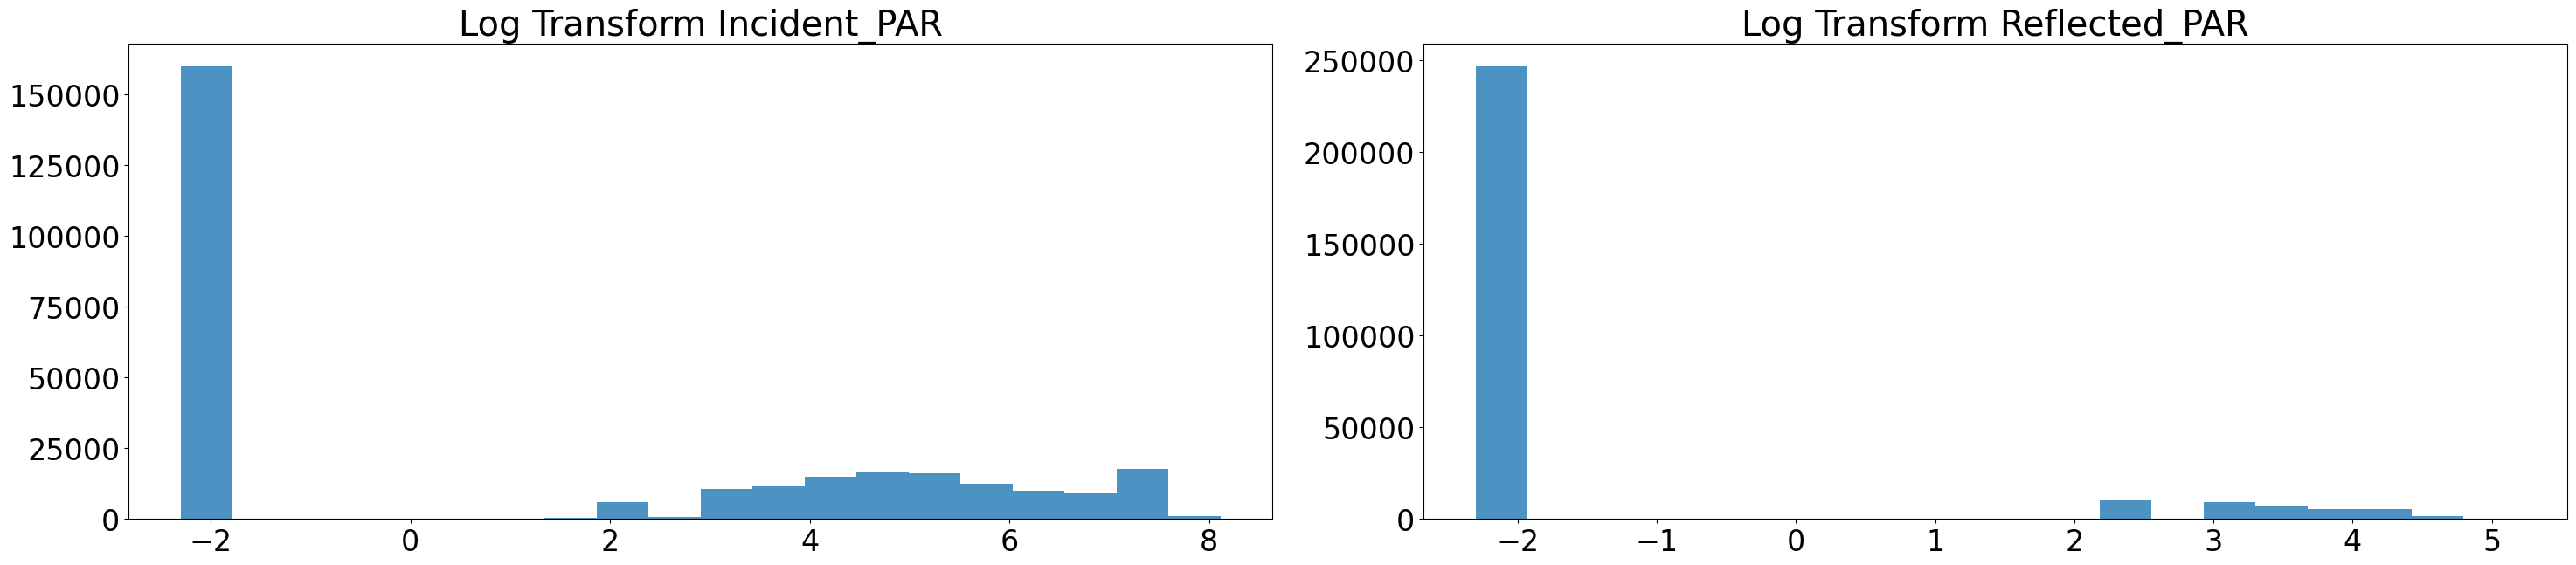
\includegraphics[width=1.0\textwidth]{Fig5_graph_critique_a.png}
\caption{PAR distribution under the log transformation}
\label{fig:graph_crtique_a}
\end{figure*}

\section{Interesting Findings}
\section{Graph Critique}
\subsection{Part a: Log Transform of Data}
We took a log transformation on the incident and the reflected PAR and plotted them. Note that since many zero values exist, we add a small positive constant to all values before taking the log.
\\ \\
\begin{figure}[h!]
\centering
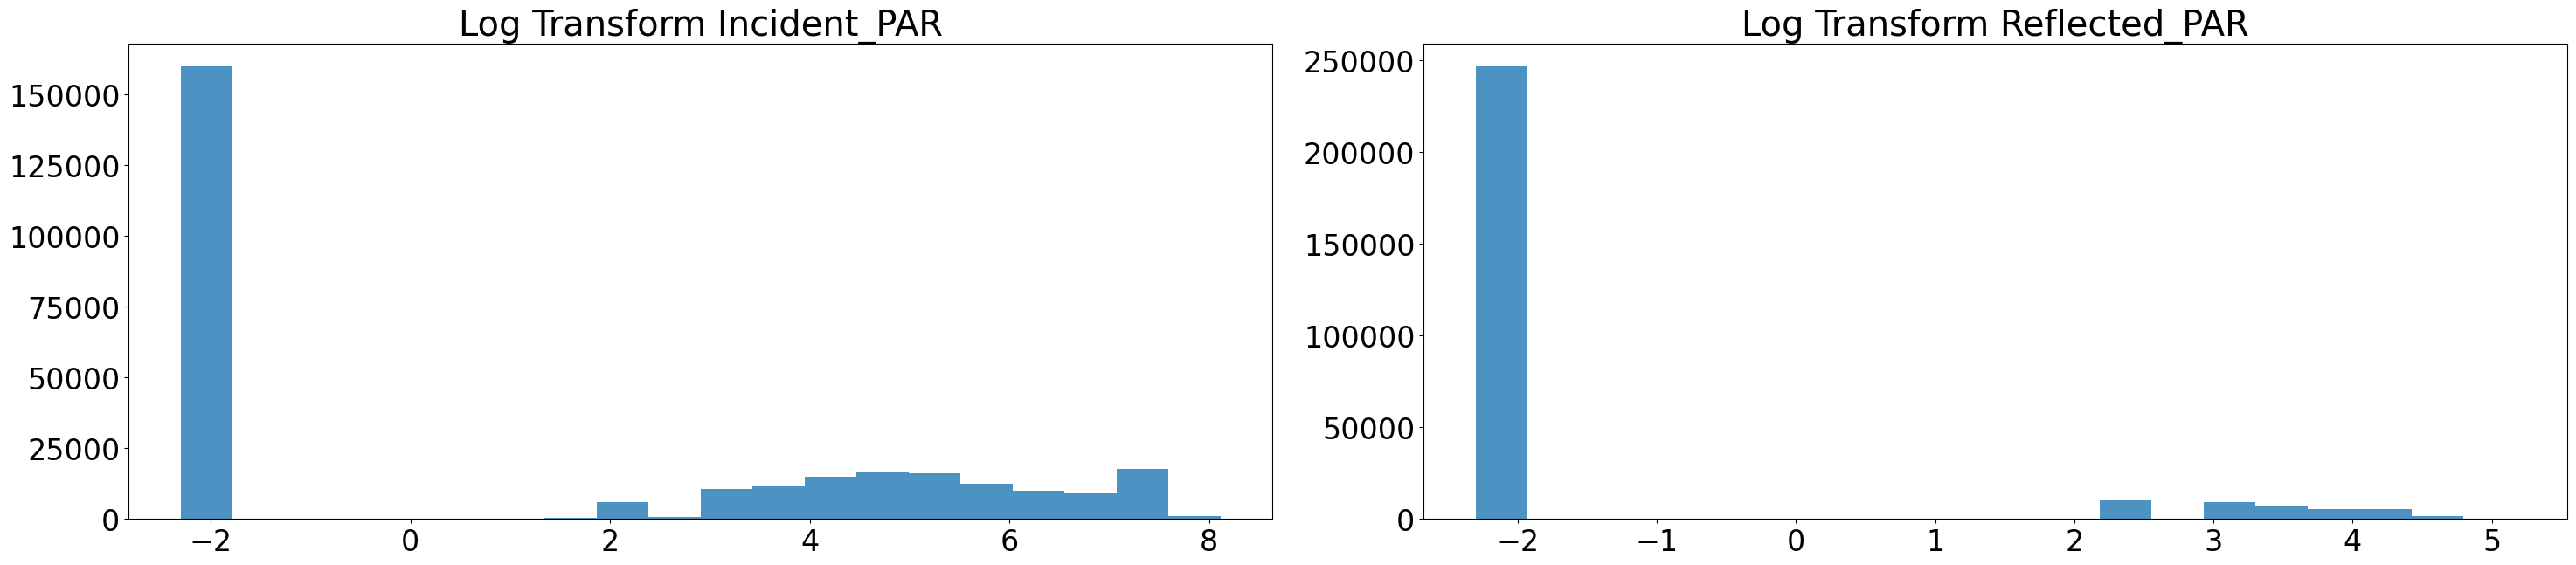
\includegraphics[width=1.0\textwidth]{Fig5_graph_critique_a.png}
\caption{PAR distribution under the log transformation}
\label{fig:graph_crtique_a}
\end{figure}
Figure \ref{fig:graph_crtique_a} shows the log-transformed Incident and Reflected PAR. We can see the large number of zero values. Aside from that, we see that the remaining non-zero log incident PAR values have a bimodal distribution, with a mode around 5 and close to 8. For reflected PAR, we see that majority of the data points are 0, with the remaining values ranging from 2-4; we see no discernible distribution here.

\subsection{Part b: Boxplot Evaluation}
We note two issues with the boxplots.
\begin{enumerate}
    \item We know there are significant variations in the data across time, hence it might be misleading to summarise all the data in a boxplot.
    \item We know that the distribution for incident PAR and reflected PAR is zero-inflated and multimodal, hence summarising in a boxplot can be misleading.
\end{enumerate}
We focus on point 2, as the author's meant to remove the time dimension in the plot. Comparing to figure 4 of the paper, we see that incident PAR and reflected PAR has many zero values at the sampled time point. This is something the boxplot representation fails to capture. \\
Instead we have plotted a similar diagram but with each boxplot replaced by a KDE plot of the values. This is plotted in Figure \ref{fig:graph_crtique_b}. Note that we have sub-sampled the heights in order to create a plot more reasonably sized plot. With the KDE we can see clearly both the large number of zeros as well as the shifting distribution of the non zero values as the height increases.
\begin{figure}[h!]
\centering
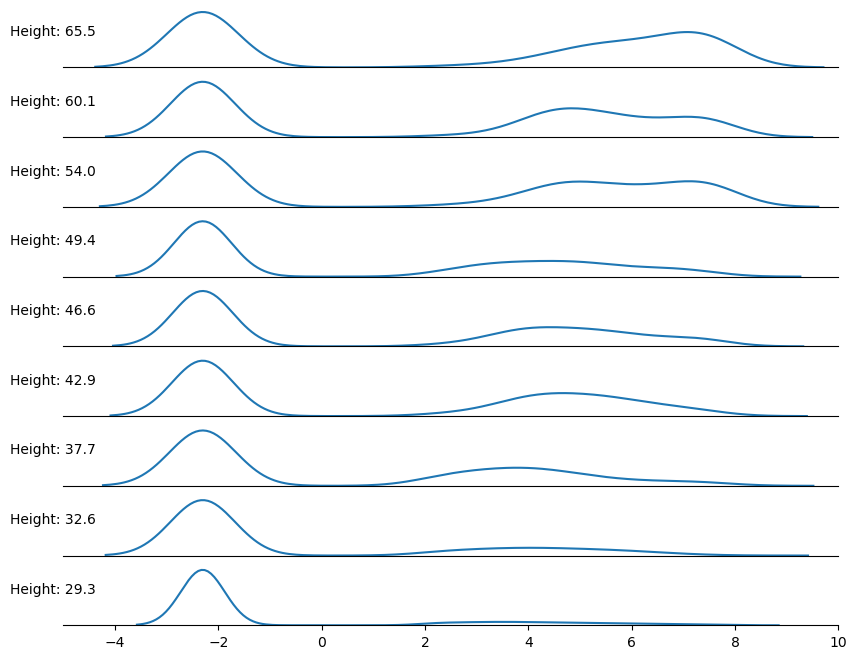
\includegraphics[width=1.0\textwidth]{Report Images/Fig7_graph_criqitue_bv2.png}
\caption{PAR distribution under the log transformation}
\label{fig:graph_crtique_b}
\end{figure}
\\

\subsection{Part c: Sequence Plot Evaluation}
The authors have plotted each node's readings with a unique color. Due to the large number of nodes, the colors are hard to distinguish and it is generally hard to pick out any trends. We consider two variations of the same plot, firstly, one where the information curve information is obscured and we plot a mean curve with estimated standard deviations, and two one where we color each curve by its height according to a color gradient.
\\
In the first variation, we color each curve by the height of its node. Generally one would use a sequential color bar to represent this information, however we have gound the sequential color bars hard to see due to large range of heights even after normalization. Hence we chose to use a diverging color bar instead. We can see from Figures \ref{fig:graph_crtique_c1} and \ref{fig:graph_crtique_c2}, that the plots now show us a very clear trend that higher up nodes have a lower humidity and higher temperature lower height nodes have a higher humidity and lower temperature.  This is new information that the previous graph of the authors were unable to showcase.
\begin{figure}[h!]
\centering
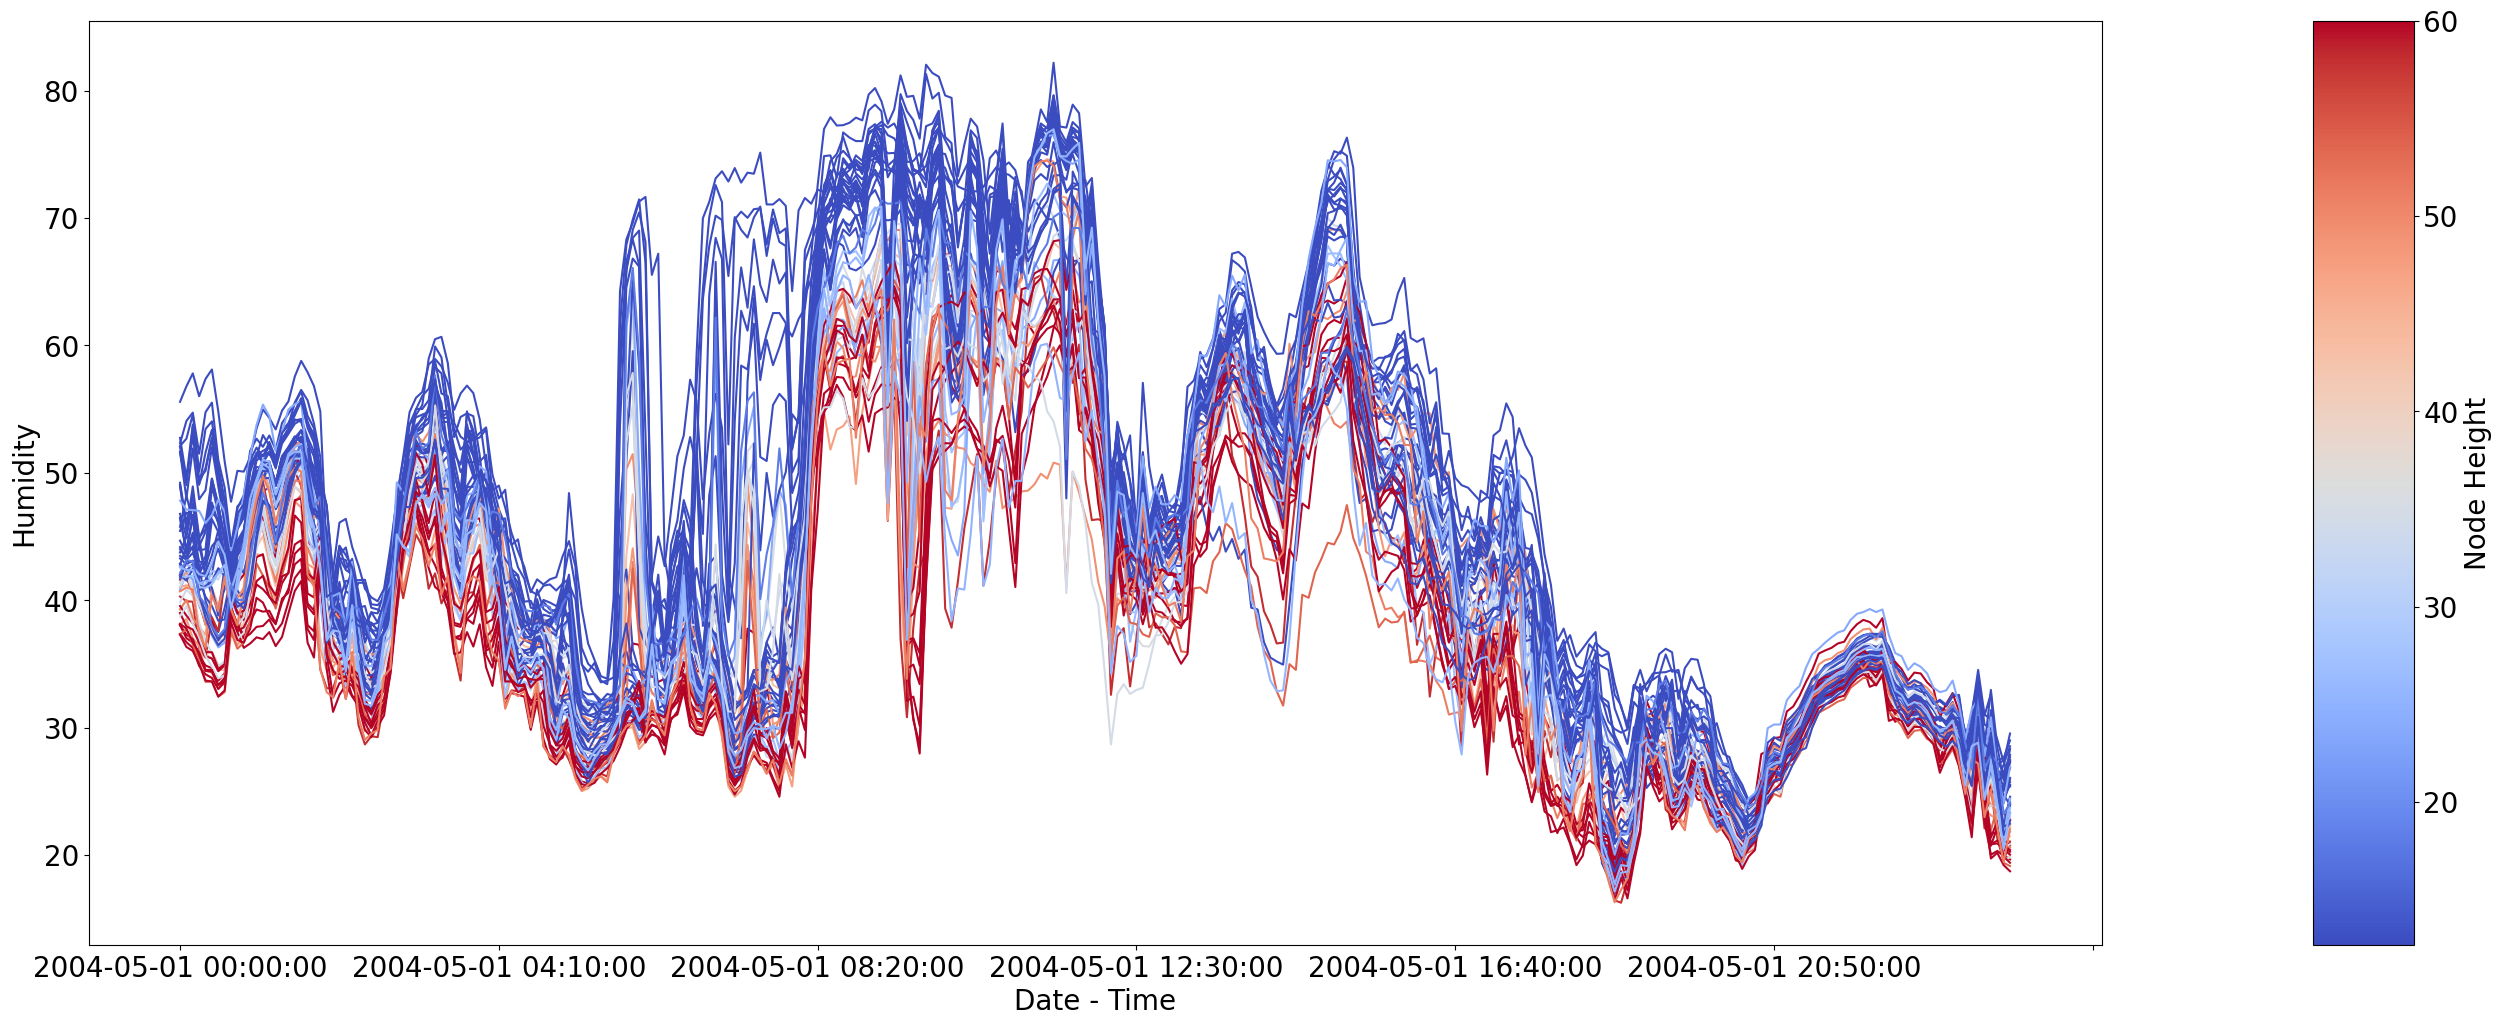
\includegraphics[width=1.0\textwidth]{Report Images/fig8_graph_critique_c1.png}
\caption{Time Series of Humidity Values Per Node with Curves Colored by Node Height}
\label{fig:graph_crtique_c1}
\end{figure}
\\
\begin{figure}[h!]
\centering
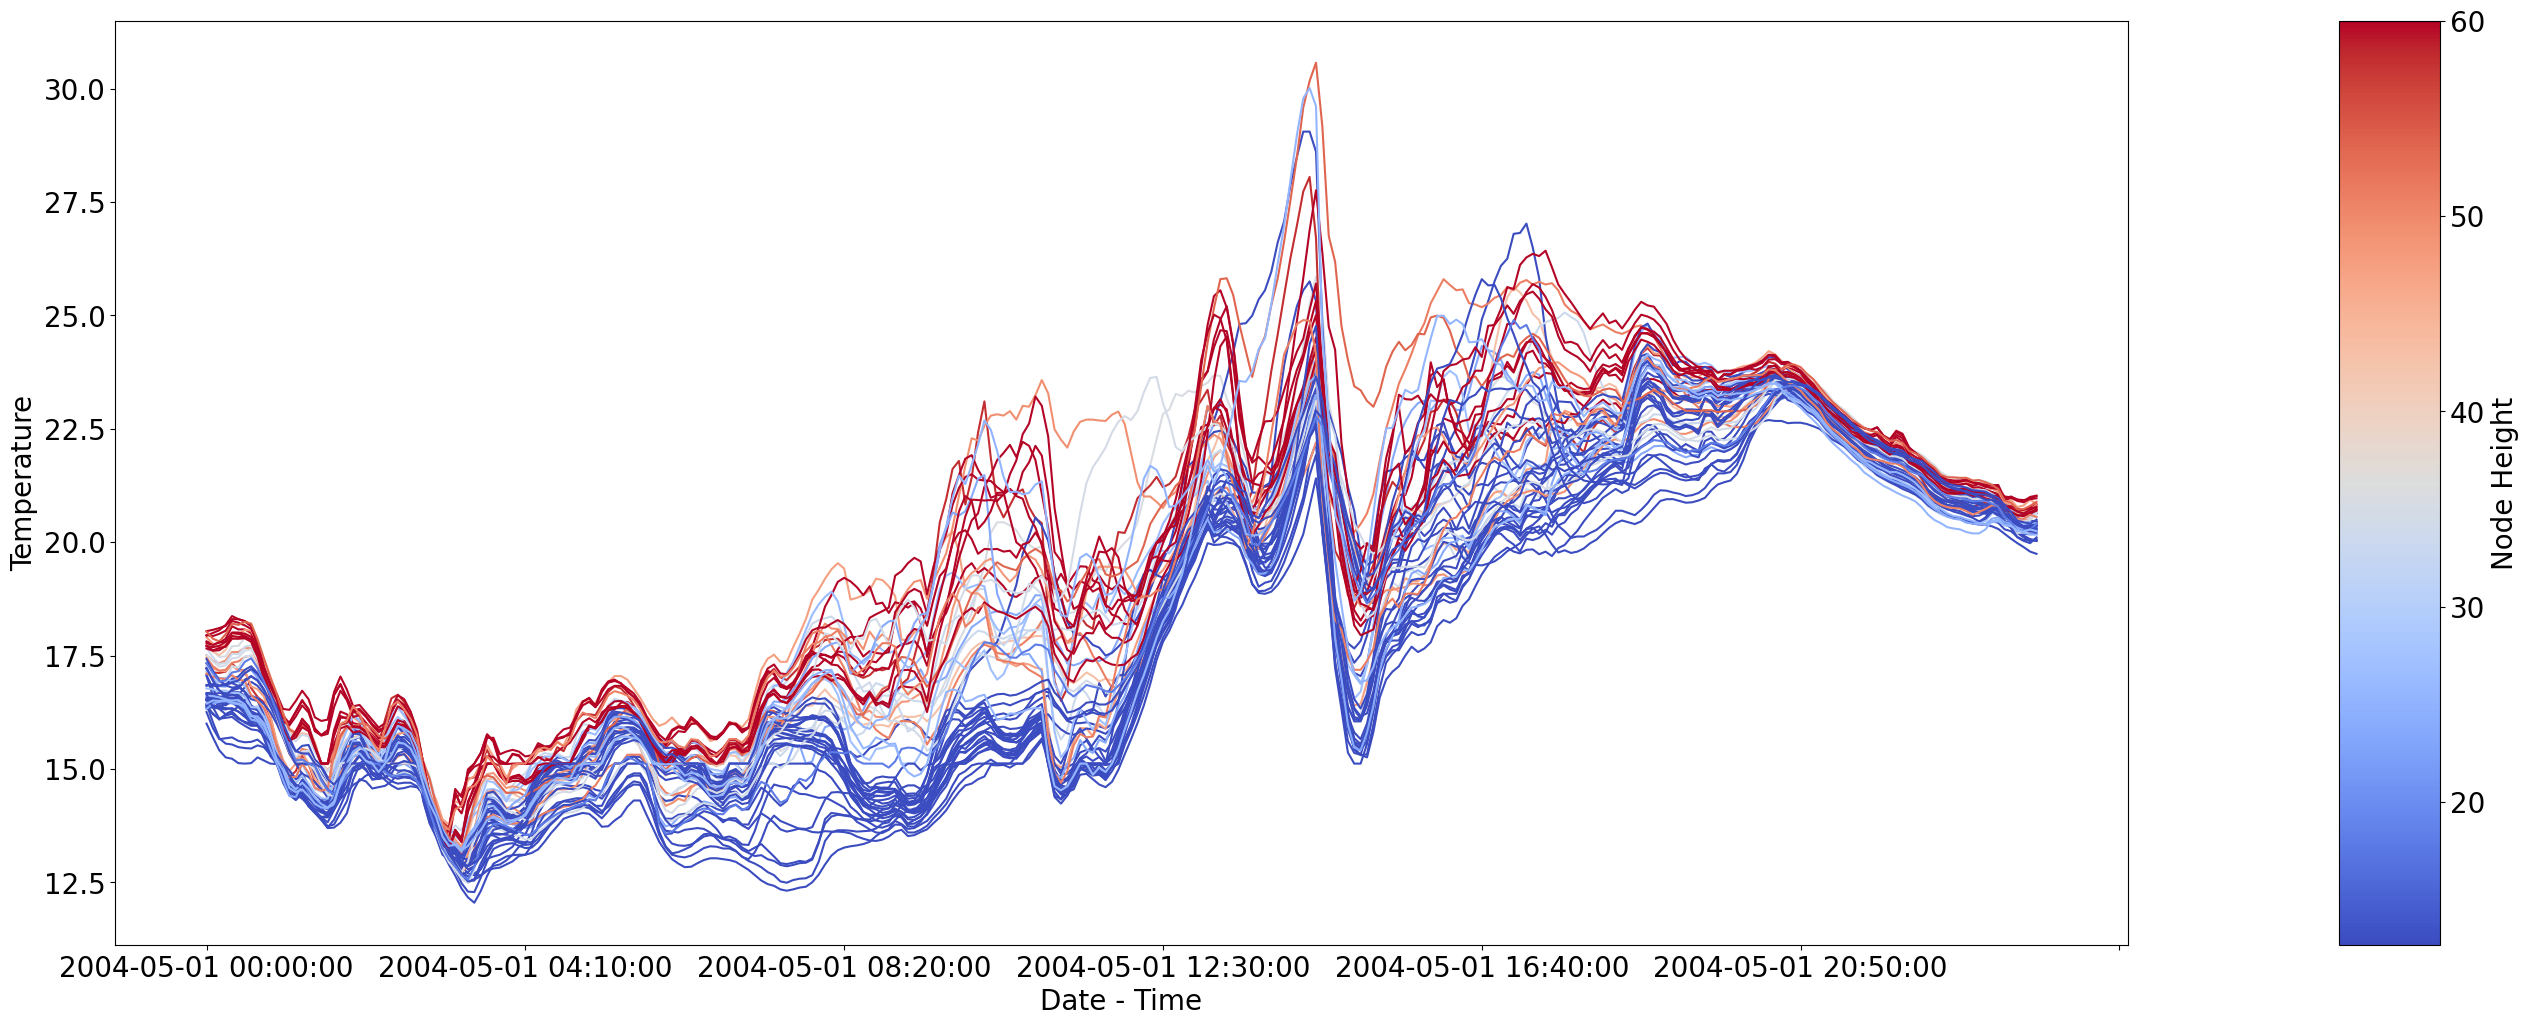
\includegraphics[width=1.0\textwidth]{Report Images/fig8_graph_critique_c2.png}
\caption{Time Series of Temperature Values Per Node with Curves Colored by Node Height}
\label{fig:graph_crtique_c2}
\end{figure}
\\

\subsection{Part d: Differences in Network and Log}

\end{document}




We saw one sensor that is consistently producing theoretically out-of-range data.

The voltage value in the logging file is different in the network dataset. Also, voltage gives out a signal on the battery life. We shall consider removing data points when the sensors are near the end of the battery life.

We have around 73 unique nodes in the logging data but only 31 on the network data.

Sometimes we can have multiple measures at the same epoch, which might also have variations within them.

Sensors have measuring error bound, so we can't mindlessly filter out the data points.


\end{document}